\chapter{Kết quả thực nghiệm, so sánh và phân tích lỗi}
\label{chap:experiments}\label{chap:results}\label{chap:comparison}
\FloatBarrier
\section{Điều kiện đánh giá chung}

So sánh dùng corpus 199.965 bài, taxonomy 20 lớp và cùng phép chia phân tầng 70/15/15, seed 42. Đối chiếu trực tiếp xác nhận mảng chỉ số train, validation và test của bốn notebook giống nhau. Trên test, toàn bộ 29.995 URL, nhãn tham chiếu và thứ tự mẫu khớp giữa ba đối chứng và metadata PhoBERT. Số lượng bằng nhau hoặc chuỗi fingerprint đơn lẻ chưa đủ cho kết luận này: PhoBERT và các đối chứng dùng cách tạo signature khác nhau.

Các số được đọc từ metrics, scores/logits, predictions, ma trận và classification report đã xuất. Tái tính từ từng hàng dự đoán xác nhận Accuracy, Macro-F1, Weighted-F1 và tổng support. Mỗi model đi vào test với duy nhất cấu hình/checkpoint đã chọn trên validation. SVM/LR được tìm trong 12 cấu hình mỗi model, BiLSTM trong ba cấu hình, PhoBERT dùng cấu hình fine-tuning ở chương~\ref{chap:training}. Ngân sách lựa chọn không bằng nhau; đây là so sánh các pipeline thực thi, không cô lập ưu thế kiến trúc.


Với lớp $c$, các chỉ số phân biệt đúng dương, sai dương và sai âm:
\begin{equation}P_c=\frac{TP_c}{TP_c+FP_c},\quad R_c=\frac{TP_c}{TP_c+FN_c},\quad F1_c=\frac{2TP_c}{2TP_c+FP_c+FN_c}.\end{equation}
Macro-F1 là $\frac1{20}\sum_c F1_c$; Weighted-F1 là $\sum_c(n_c/N)F1_c$. Accuracy là tỷ lệ đúng toàn tập. Mẫu số bằng không nhận 0; micro-F1 bằng Accuracy trong phân loại đơn nhãn đầy đủ lớp. Một kết quả cao theo số lượng chưa bảo đảm các lớp nhỏ có chất lượng tương ứng.


\subsection{Điều kiện đối chiếu từng bài}
Cùng số lượng test không đủ cho một phép so sánh ghép cặp. Metadata có article index, URL và label ID; dự đoán được đối chiếu bằng khóa này trước khi tính số model cùng đúng. Một hoán vị đúng của nhãn và dự đoán vẫn có thể cho điểm tổng đúng, nhưng nếu ghép sai thứ tự giữa model thì số lỗi chung và bootstrap chênh lệch sẽ sai. Audit vì vậy kiểm tra cả mảng split, các URL và từng hàng nhãn, không chỉ ba scalar metric.

Phần so sánh chính dùng argmax score/logit của bốn pipeline, không dùng nhãn cuối sau hệ số PhoBERT để tăng riêng một dòng. Temperature dương giữ thứ tự score nên có thể đánh giá calibration mà không đổi giao thức nhãn. Accuracy, Macro-F1 và Weighted-F1 là thuộc test cuối; các điểm validation trong bảng cấu hình chỉ giải thích quyết định lựa chọn. Không coi chúng như hai lần đánh giá test độc lập.

\FloatBarrier
\section{Kết quả tổng thể bốn phương pháp}

\DataTable{tables/comparison_primary.tex}{Chất lượng bốn model với quyết định argmax score/logit; chưa dùng hệ số điều chỉnh lớp của PhoBERT. Chỉ số phần trăm, làm tròn bốn chữ số trên cùng 29.995 bài test.}
PhoBERT đạt Macro-F1 87,22\%, SVM 85,33\%, LR 84,98\% và BiLSTM 84,60\%. Khoảng cách PhoBERT--SVM là 1,89 điểm phần trăm Macro-F1 và 1,17 điểm Accuracy, tương ứng 350 bài đúng ròng. SVM có 26.970 bài đúng, so với 26.714 của LR và 26.595 của BiLSTM. Những giá trị này là kết quả corpus hiện tại, không lấy từ bảng nghiên cứu ở chương~\ref{chap:related}.

Temperature dương không đổi argmax ở cả bốn model. Riêng hệ số lớp của PhoBERT thay nhãn sau temperature, nâng Accuracy từ 91,08\% lên 91,13\% và Macro-F1 từ 87,22\% lên 87,25\%, đạt 27.333 bài đúng. Trạng thái này phục vụ ứng dụng ở Phụ lục~\ref{app:application}; không dùng thay dòng argmax trong đối chứng chính.

Kết quả cho thấy TF--IDF toàn văn đã cung cấp đối chứng mạnh. BiLSTM học từ đầu chưa vượt hai mô hình tuyến tính trong cấu hình đã khảo sát. Điều đó không chứng minh thứ tự từ vô ích, LSTM nói chung kém hơn SVM, hay toàn bộ mức tăng của PhoBERT đến từ pretraining. Cách cắt, stopword, lặp tiêu đề, trọng số lớp và ngân sách tối ưu đều là biến đồng thời thay đổi.


\begin{table}[htbp]\centering\small\caption{PhoBERT trước/sau điều chỉnh theo lớp trên cùng test; chỉ số ở thang 0--1, chênh lệch là sau trừ trước.}\label{tab:pho_adjustment}
\begin{tabularx}{\linewidth}{>{\raggedright\arraybackslash}Xrrr}
\toprule
Chỉ số & Trước & Sau & Chênh lệch\\\midrule
Accuracy & 0.910818 & 0.911252 & 0.000433\\
Weighted-F1 & 0.911176 & 0.911450 & 0.000273\\
Macro-F1 & 0.872191 & 0.872529 & 0.000337\\
\bottomrule\end{tabularx}
\end{table}
Theo nhãn đã lưu, PhoBERT đúng 27.320 bài trước và 27.333 bài sau điều chỉnh. Quy tắc sửa đúng 112 bài nhưng đổi thành sai 99 bài; ròng tăng 13/29.995 bài. Macro-F1 tăng 0,0337 điểm phần trăm, là mức nhỏ và không chứng minh lợi ích ổn định ở mọi lớp hoặc lần huấn luyện. Temperature riêng không tạo mức tăng này vì argmax của nó giữ nguyên.


\subsection{Đọc chênh lệch tổng thể}
Macro-F1 trung bình ngang nhau giữa các lớp, nên khoảng cách thể hiện cả những chuyên mục ít bài mà Accuracy có thể làm mờ. Weighted-F1 tăng trọng lượng lớp đông; khoảng cách giữa hai F1 là một tín hiệu cần phân tích theo lớp, không một công thức đo mất cân bằng duy nhất. Hai model có cùng Accuracy cũng có thể phân bố lỗi khác nhau và đạt Macro-F1 khác. Vì vậy, bảng tổng không xác định lớp nào cần rà soát.

PhoBERT dẫn đầu trong cả ba chỉ số argmax của snapshot, nhưng SVM vẫn gần và fit được trên CPU. Kết quả này làm baseline từ vựng trở thành đối chứng thực chất, thay vì chỉ một mức tham chiếu dễ vượt. Ngược lại, BiLSTM chưa vượt SVM/LR không chứng minh embedding chuỗi không hữu ích: nó học từ đầu, dùng một tầng recurrent, giữ chuỗi giới hạn và có ngân sách ứng viên khác. Tên họ mô hình không thay thế cấu hình cụ thể đã đánh giá.

Mức tăng sau hệ số lớp cần đọc như một đổi quy tắc quyết định của cùng PhoBERT. Số bài đúng ròng bằng sửa đúng trừ đổi sai; nó không cho thấy 112 trường hợp là lợi ích mà bỏ qua 99 trường hợp bị hại. Tăng Macro-F1 nhỏ cũng không bảo đảm các luồng nghiệp vụ được cải thiện như nhau. Test chỉ mô tả tác động của tham số đã chọn trên validation, không dùng chọn lại các hệ số để tối đa hóa kết quả cuối.

\FloatBarrier
\section{Kết quả theo 20 chuyên mục}

\DataTable{tables/comparison_per_class.tex}{F1 (\%) theo 20 chuyên mục với argmax, cùng support test; DTTS là Dân tộc thiểu số. Giá trị làm tròn có thể che chênh lệch rất nhỏ.}
Thể thao, Thế giới và Ô tô -- Xe máy đạt F1 cao ở cả bốn pipeline. SVM và PhoBERT đều khoảng 98,78\% ở Thể thao; khác biệt tại chữ số nhỏ không đủ để coi một model tốt hơn có ý nghĩa theo lớp này. Ngược lại, Dân tộc thiểu số và miền núi đạt 69,38\% với PhoBERT, cao hơn mức 58,06--59,53\% của ba đối chứng. Nội dung chuyên đề đạt 79,74\% với PhoBERT, so với 74,18--76,57\%. Lợi thế tổng thể vì vậy không phân bố đều trên mọi chuyên mục.

\subsection{Nông thôn mới: đánh đổi precision và recall}
\DataTable{tables/comparison_rare.tex}{Nông thôn mới: precision, recall và F1 của bốn model trước điều chỉnh nhãn; support là 146 bài.}
BiLSTM đạt F1 48,24\%, LR 47,06\%, PhoBERT argmax 45,57\% và SVM 39,53\%. Ngay cả PhoBERT sau điều chỉnh lớp đạt 46,39\%, vẫn thấp hơn hai giá trị đầu trong mẫu test này. SVM nhận đúng 51/146 bài, LR 80, BiLSTM 89 và PhoBERT argmax 72. Recall cao hơn của BiLSTM đi kèm precision chỉ 39,91\%; đây không phải cải thiện đồng thời mọi tiêu chí.

Ma trận cho thấy SVM chuyển 86 bài Nông thôn mới sang Nội dung chuyên đề. Ở chiều ngược, LR chuyển 106 bài Nội dung chuyên đề sang Nông thôn mới, BiLSTM chuyển 128 bài. Những lỗi từ lớp lớn góp phần làm precision của lớp hiếm thấp. Trọng số loss, số mẫu và đặc điểm nội dung cùng ảnh hưởng ranh giới; chưa có ablation để xác định nguyên nhân riêng. Với 146 mẫu, thứ hạng F1 theo lớp cần được kiểm chứng trên nhiều seed và một tập gán nhãn được rà soát.


Các lớp được định nghĩa không cùng một kiểu: có nhãn lĩnh vực như Thể thao, có nhãn bình luận như Tuần Việt Nam, và có chuyên đề/chính sách. Một vector từ vựng có thể đặc trưng rõ lĩnh vực nhưng khó nhận ra quyết định tổ chức xuất bản. Tương tự, encoder ngữ cảnh không được cung cấp breadcrumb để phân biệt một bài đăng theo chuyên đề với bài cùng nội dung ở mục khác. Đây là giới hạn của mục tiêu suy chuyên mục chỉ từ title/content, không phải bằng chứng model đã đọc sai toàn bộ ngữ nghĩa.

Điều chỉnh hệ số PhoBERT không đồng thời cải thiện mọi lớp. Nông thôn mới tăng từ 45,57\% lên 46,39\%, còn Dân tộc thiểu số và miền núi giảm từ 69,38\% xuống 68,77\%. Tối ưu Macro-F1 validation là đánh đổi toàn cục, không cam kết precision/recall của từng lớp test tăng. Các hệ số nằm trong artifact, không chọn lại theo test để làm đẹp bảng.



\subsection{Lợi thế không phân bố đều giữa các chuyên mục}
Hai model đạt F1 gần bằng nhau ở lớp dễ chưa có nghĩa chúng đúng trên cùng từng bài. F1 tổng hợp TP, FP và FN, không giữ danh sách URL; số đúng chung và đúng riêng trong phân tích ghép cặp bổ sung thông tin này. Do đó, không chọn một model để thay toàn bộ model khác chỉ vì vài lớp có số làm tròn bằng nhau. Cũng không coi lợi ích ensemble là đã xác nhận từ việc các lỗi khác nhau.

Nhóm Thể thao, Thế giới và Ô tô -- Xe máy có điểm cao ở nhiều biểu diễn, trong khi Nội dung chuyên đề và các nhãn dân tộc phân tách mạnh hơn. Pattern này giúp đặt giả thuyết về mức tập trung từ vựng và ranh giới xuất bản. Nó không tự định lượng tác động phần giữa bị cắt vì chưa có so sánh head-only/Head--Tail/chunked trong cùng model. Cách diễn giải giữ ranh giới giữa quan sát theo lớp và nguyên nhân cần thí nghiệm thêm.

Một lớp lớn có thể tạo nhiều false positives cho một lớp nhỏ dù tỷ lệ nhầm trên hàng của lớp lớn thấp. Đây là lý do cần xem cả chiều đi và chiều về trong confusion, thay vì chỉ chọn ô có màu đậm. Với Nông thôn mới--Nội dung chuyên đề, support hai bên rất khác, nên recall lớp hiếm và precision của dự đoán lớp hiếm phụ thuộc hai nguồn mẫu số khác nhau. Phân tích P/R ở bảng lớp hiếm giúp tránh gọi một sự tăng dự đoán đơn thuần là chất lượng tăng đồng đều.

Kết quả theo nhãn cũng không cung cấp hiệu năng cho một nhãn mới chưa xuất hiện trong taxonomy. Một bài thuộc lĩnh vực mới hoặc một mục con đổi cách tổ chức vẫn bị ép vào một trong 20 đầu ra nếu đưa vào classifier. Top-$k$ mở thêm ứng viên cho người rà soát, không biến bài toán thành mô hình multi-label hoặc zero-shot. Những giới hạn này cần được giữ khi chuyển từ đánh giá chuyên mục sang sử dụng gợi ý nhãn.


\subsection{Support và ranh giới nhãn}
Với Nông thôn mới, recall trả lời bao nhiêu bài của lớp thật được nhận ra, còn precision trả lời bao nhiêu bài được gọi là lớp này thực sự thuộc lớp. Tăng lượng dự đoán có thể tăng recall nhưng hút bài của Nội dung chuyên đề vào, làm precision thấp. F1 kết hợp hai phía; không chọn một chiều để tuyên bố model ``giải quyết lớp hiếm''. Với support 146, một số nhỏ bài đổi nhãn cũng làm chỉ số biến động rõ.

Những lớp dân tộc cho thấy nguồn khó khác với Nông thôn mới. Cùng bài về chính sách, du lịch hoặc văn hóa địa phương có thể xuất hiện trong các khuôn chuyên mục khác nhau. Bước xác minh breadcrumb ngăn lấy nhãn của trang danh sách nhầm, nhưng không cung cấp feature này cho model test. Vì vậy, dataset đúng chính sách nhãn và model khó học nhãn từ văn bản có thể đồng thời tồn tại.

Các lớp tập trung như Thể thao hay Ô tô -- Xe máy có nhiều dấu hiệu thuật ngữ, nhưng điểm cao chưa chứng minh một thuật ngữ riêng gây ra dự đoán. Còn với chuyên mục bình luận, tín hiệu có thể nằm ở giọng điệu, cấu trúc hoặc cách xuất bản mà vector n-gram và chuỗi đã cắt giữ không đầy đủ. Các giả thuyết này chỉ định nơi cần đọc lỗi và ablation, không được trình bày như kết quả nhân quả đã đo.

\FloatBarrier
\section{Ma trận nhầm lẫn và phân tích lỗi bài thật}
Hàng ma trận là nhãn tham chiếu, cột là nhãn dự đoán; tổng hàng bằng support và toàn ma trận bằng 29.995. Chuẩn hóa theo hàng cho biết phân bố dự đoán khi biết lớp thực, khác precision của nhãn được chọn. ID đối chiếu bảng~\ref{tab:class_split}; ma trận của ba baseline nằm ở Phụ lục~\ref{app:evidence}.
\begin{figure}[tbp]\centering
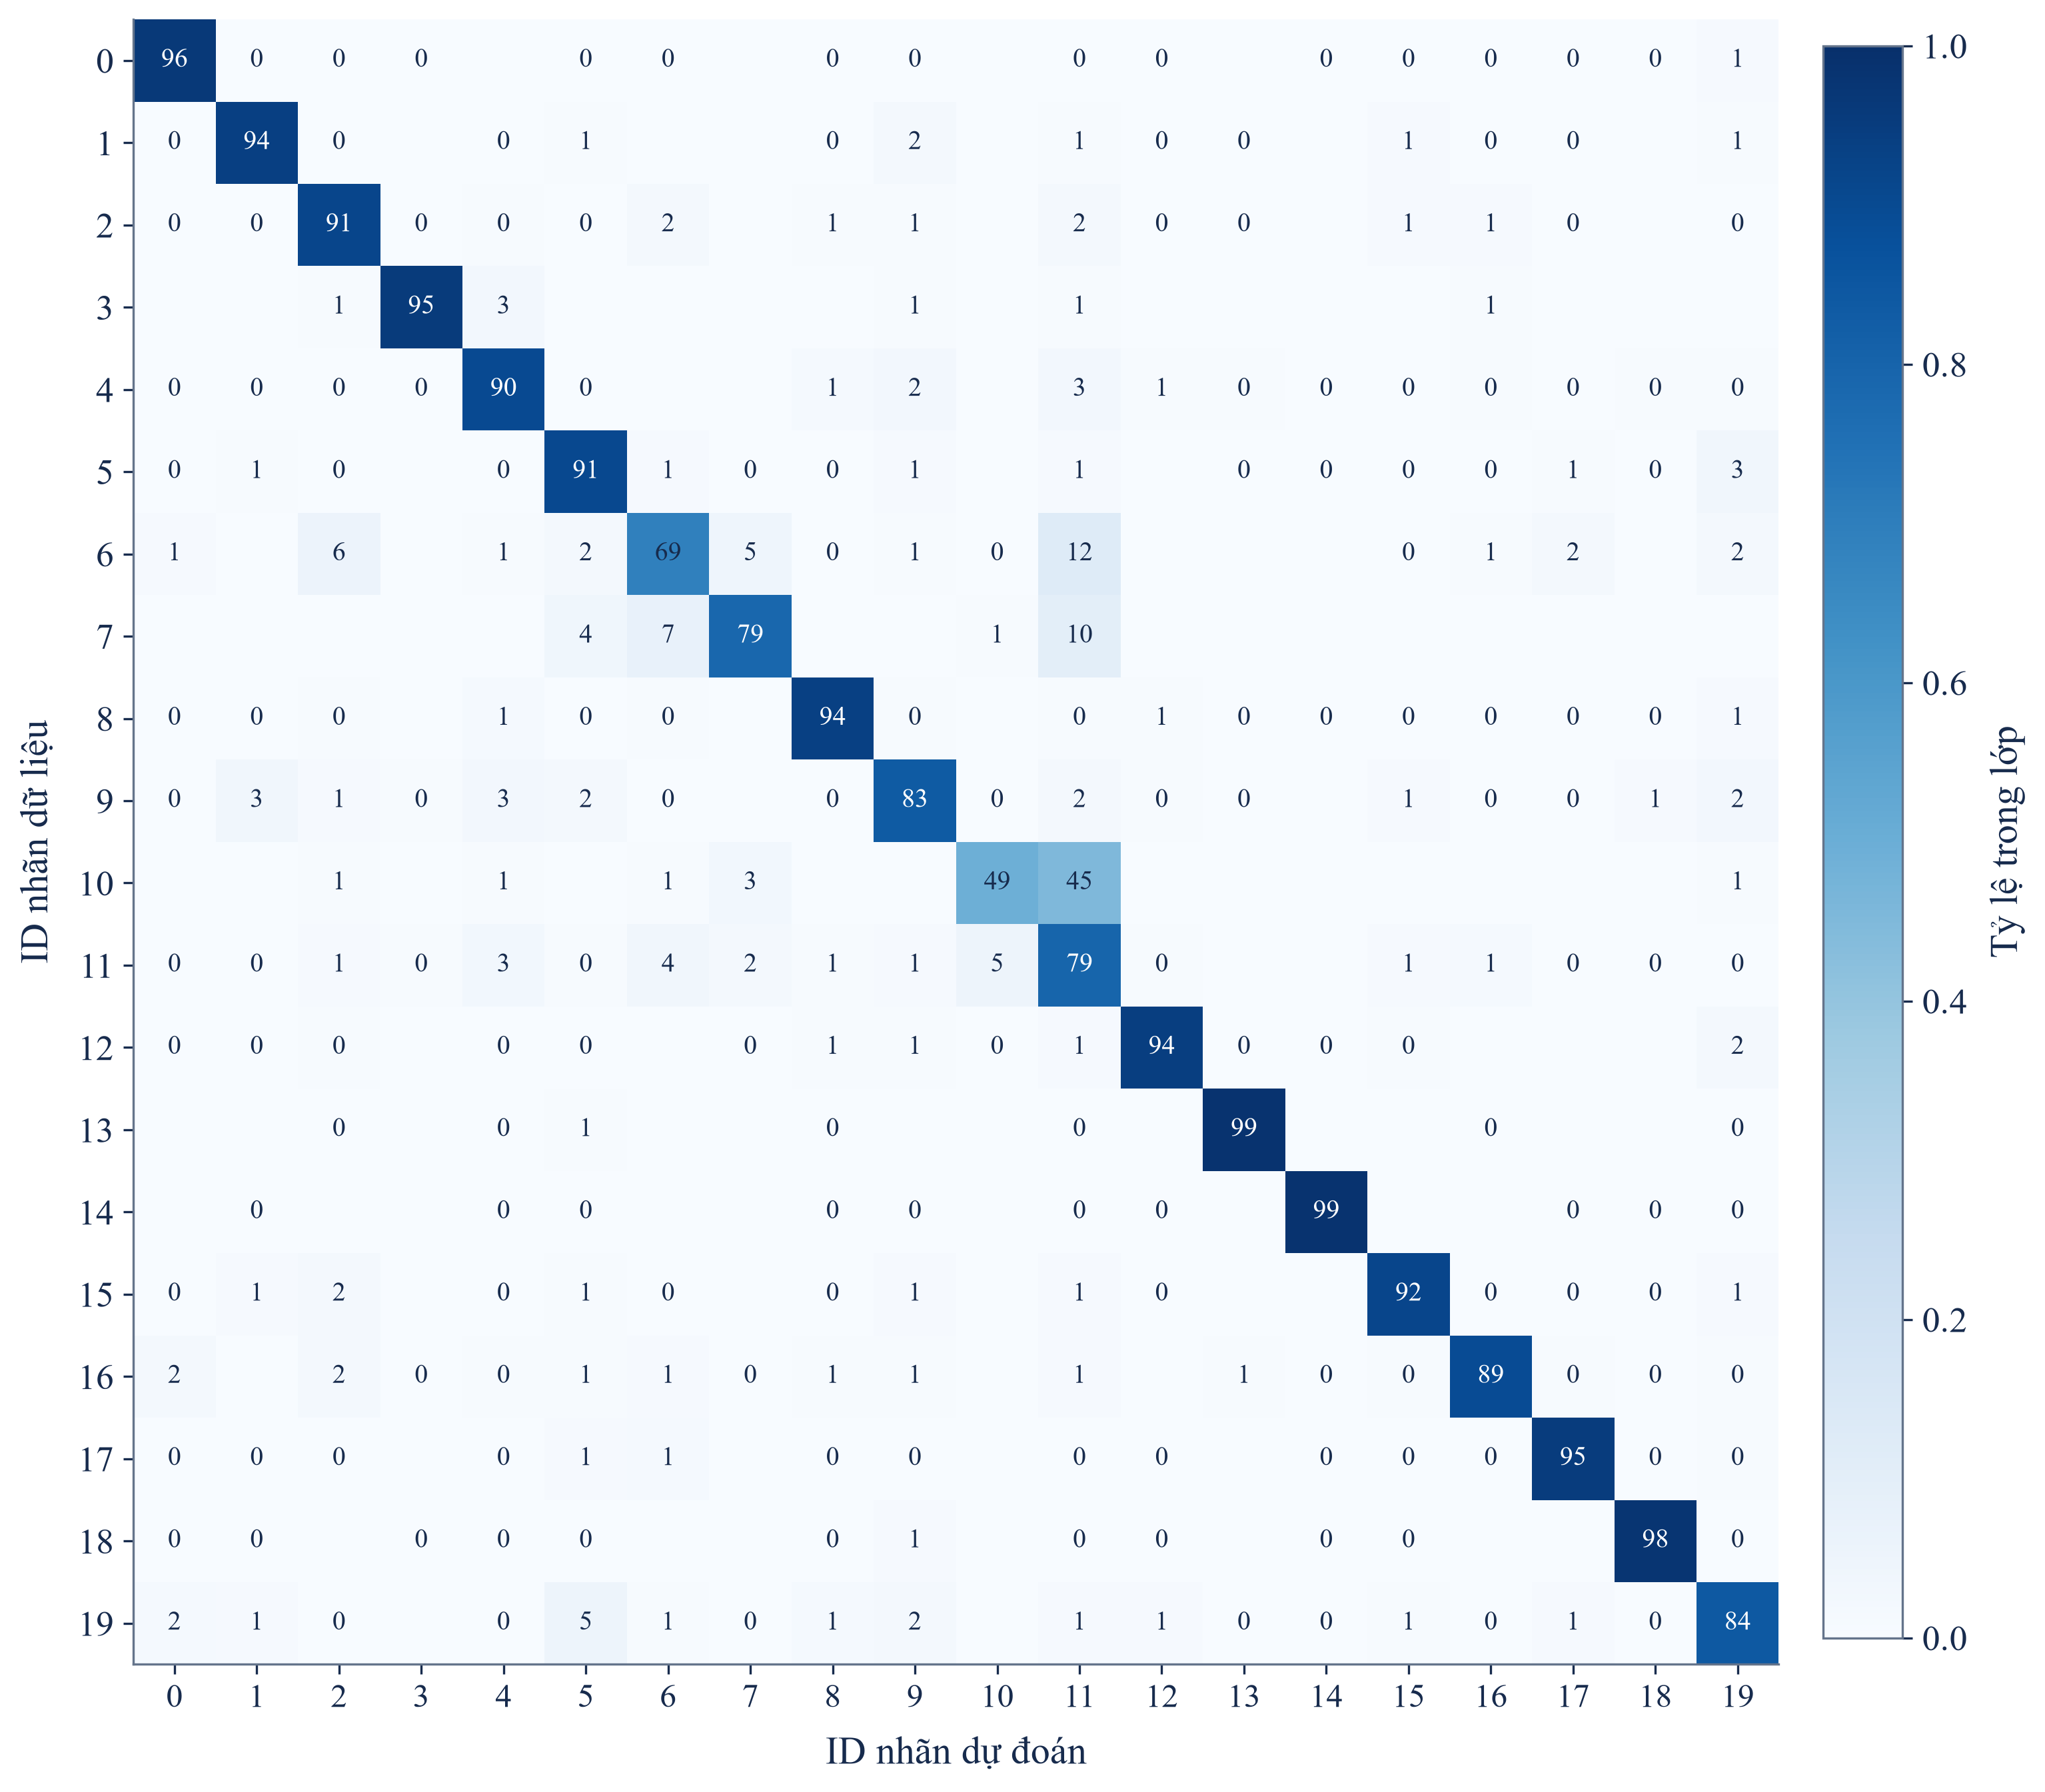
\includegraphics[width=.96\textwidth,height=.72\textheight,keepaspectratio]{assets/evaluation/confusion_before_normalized.png}
\caption{PhoBERT chuẩn hóa theo hàng, argmax trước hệ số lớp; thang tỷ lệ 0--1.}\label{fig:phobert-confusion-main}\end{figure}
\begin{table}[htbp]\centering\small\caption{Các hướng nhầm nổi bật của PhoBERT argmax; tỷ lệ lấy support nhãn tham chiếu làm mẫu số.}\label{tab:confusions_main}
\begin{tabularx}{\linewidth}{>{\raggedright\arraybackslash}X>{\raggedright\arraybackslash}Xrr}
\toprule
Nhãn tham chiếu & Nhãn dự đoán & Số bài & Tỷ lệ hàng\\\midrule
Nội dung chuyên đề & Nông thôn mới & 94 & 4,99\%\\
Đời sống & Du lịch & 87 & 4,88\%\\
Dân tộc - Tôn giáo & Nội dung chuyên đề & 68 & 12,25\%\\
Nội dung chuyên đề & Dân tộc - Tôn giáo & 66 & 3,50\%\\
Nông thôn mới & Nội dung chuyên đề & 66 & 45,21\%\\
Kinh doanh & Bất động sản & 61 & 3,22\%\\
Nội dung chuyên đề & Công nghệ & 56 & 2,97\%\\
Du lịch & Đời sống & 56 & 3,40\%\\
\bottomrule\end{tabularx}
\end{table}
Nông thôn mới bị chuyển sang Nội dung chuyên đề ở 66/146 bài, trong khi chiều ngược có 94/1.885 bài. Cùng lượng từ về địa phương, sinh kế và chương trình phát triển có thể xuất hiện ở cả hai lớp; hướng nhầm không đối xứng do khác support và ranh giới model. Đời sống--Du lịch, Kinh doanh--Bất động sản cũng có vùng giao thoa, nhưng ma trận chưa cho biết thiếu phần giữa bài, mất chữ số hay nhãn biên tập là nguyên nhân riêng.


\DataTable{tables/comparison_shared_errors.tex}{Số model dự đoán đúng từng bài trong bốn quyết định argmax; tổng bằng 29.995.}
Cả bốn model cùng đúng ở 24.677 bài và cùng sai ở 1.251 bài. Trong nhóm cùng sai, Nội dung chuyên đề có 186 bài, Kinh doanh 169 và Đời sống 156; Nông thôn mới có 24/146 bài, Dân tộc -- Tôn giáo 83/555 bài. Số tuyệt đối và tỷ lệ trong lớp thể hiện hai mặt khác nhau của độ khó, không được dùng thay nhau.

Ba ví dụ chung có thể truy vết từ artifact: ``Google tích hợp AI Gemini vào hệ sinh thái sản phẩm'' có nhãn Giáo dục nhưng cả bốn dự đoán Công nghệ; ``The Sonata -- sống tận hưởng tại `tọa độ quốc tế' bên sông Hàn'' có nhãn Kinh doanh nhưng cả bốn chọn Bất động sản; ``Ô tô mới có thể được miễn đăng kiểm lần đầu từ năm 2023'' có nhãn Thời sự nhưng cả bốn chọn Ô tô -- Xe máy. URL tương ứng là:
\begin{itemize}
\item \href{https://vietnamnet.vn/google-tich-hop-ai-gemini-vao-he-sinh-thai-san-pham-2281849.html}{VietNamNet, bài 2281849: Google tích hợp AI Gemini};
\item \href{https://vietnamnet.vn/the-sonata-song-tan-huong-tai-toa-do-quoc-te-ben-song-han-2348982.html}{VietNamNet, bài 2348982: The Sonata bên sông Hàn};
\item \href{https://vietnamnet.vn/o-to-moi-co-the-duoc-mien-dang-kiem-lan-dau-tu-nam-2023-2094970.html}{VietNamNet, bài 2094970: Miễn đăng kiểm lần đầu}.
\end{itemize}
Những trường hợp này cho thấy nhãn chuyên mục có thể phụ thuộc cách tổ chức biên tập hơn tên chủ đề dễ nhận thấy. Không tự đổi nhãn tham chiếu vì nhiều model đồng ý với nhau. Cần rà soát bài gốc, quy tắc taxonomy và bằng chứng chuyên mục trước khi kết luận nhãn sai hoặc model sai theo nghĩa ngữ nghĩa.


Các ví dụ trên được chọn theo giao thức argmax chung; không trộn nhãn sau hệ số PhoBERT vào lỗi bốn model. Việc nhiều model cùng sai có thể do tín hiệu chủ đề nổi bật, cách cắt hoặc cùng khó với taxonomy. Để phân biệt, cần kiểm toán bài và nhãn thay vì đổi ground truth theo đa số dự đoán.


\subsection{Diễn giải các ví dụ có thể truy vết}
Ở bài Gemini, chủ thể Google và sản phẩm AI cung cấp tín hiệu rõ cho Công nghệ, trong khi nhãn tham chiếu là Giáo dục. Việc cả bốn chọn cùng một lớp phù hợp với tiêu đề chưa đủ kết luận nhãn gốc sai: cần đọc nội dung và bối cảnh chuyên mục. Đây là ví dụ ranh giới giữa chủ đề nổi bật trong văn bản và mục xuất bản, đúng với định nghĩa tác vụ đơn nhãn đã nêu.

Bài The Sonata có nhãn Kinh doanh nhưng dự đoán chung Bất động sản, minh họa vùng nội dung giao thoa giữa giới thiệu dự án và hoạt động doanh nghiệp. TF--IDF toàn văn lẫn hai mô hình chuỗi đều gặp lỗi, nên không thể giải thích riêng bằng việc PhoBERT bỏ phần giữa. Điều này cũng chưa chứng minh cách cắt vô hại: các model có thể cùng sai vì những lý do khác nhau, dù nhãn cuối giống nhau.

Bài miễn đăng kiểm có nhãn Thời sự và cùng dự đoán Ô tô -- Xe máy. Đơn vị phương tiện, quy định đăng kiểm và năm xuất bản có thể tạo tín hiệu lĩnh vực cạnh tranh với loại tin thời sự; mô hình chuẩn hóa còn bỏ dãy số. Không có thí nghiệm giữ chữ số để xác định tác động của bước này. Ba ví dụ được chọn có chủ đích, không đại diện tỷ lệ của từng kiểu lỗi trong toàn corpus.


\subsection{Sai số do mục tiêu đơn nhãn và quan sát đầu vào}
Nhãn chuyên mục chỉ giữ một quyết định dù bài có nhiều lĩnh vực. Một model có thể nhận ra chủ đề dễ thấy nhưng vẫn sai mục tiêu xuất bản, như các ví dụ Kinh doanh--Bất động sản hoặc Thời sự--Ô tô. Ngược lại, model khớp nhãn không có nghĩa nó hiểu mọi chi tiết bài báo. Accuracy của chuyên mục vì vậy không đo tính đúng của nội dung, khả năng đọc hiểu hoặc chất lượng thông tin.

URL và breadcrumb rất hữu ích xác minh dữ liệu, nhưng đưa chúng vào feature sẽ đổi bài toán sang khai thác chính cấu trúc xuất bản. Project giữ chúng ngoài classifier để đánh giá dự đoán từ văn bản. Chính lựa chọn đầu vào này tạo một giới hạn học được khi taxonomy dùng tín hiệu không hiện rõ trong title/content. Khi đề xuất cải tiến, cần quyết định có giữ nguyên nhiệm vụ không, thay vì âm thầm thêm feature rồi đối chiếu điểm như cùng điều kiện.

Trích xuất cũng là một bước trước mô hình: lỗi thiếu đoạn, lẫn nội dung liên quan hoặc ghép từ có thể làm văn bản khác bài gốc. Các kiểm tra không rỗng và chuyên mục hợp lệ ngăn một số lỗi cấu trúc, chưa bảo đảm chất lượng toàn văn. Nếu lỗi trích xuất tồn tại ở cùng bản ghi, bốn pipeline có thể cùng chịu ảnh hưởng. Audit mẫu khó nên xem nguồn văn bản trước khi quy lỗi cho encoder.


\subsection{Từ lỗi chung tới kiểm toán dữ liệu}
Nhóm cùng sai là điểm bắt đầu cho kiểm toán vì không model nào trong bốn cấu hình sửa được bằng cơ chế hiện có. Tuy nhiên, đồng thuận sai không là một bộ gán nhãn thay thế. Để phân loại nguyên nhân, cần xem trích xuất có thiếu/ghép nhầm đoạn không, breadcrumb có quy đúng nhãn cha không và văn bản có đủ thông tin phân biệt mục hay không. Mỗi nguyên nhân dẫn đến hành động khác: sửa bản ghi, làm rõ taxonomy hoặc bổ sung mẫu học.

Một nhãn có nhiều bài cùng sai theo số tuyệt đối có thể chỉ vì support lớn. Tỷ lệ cùng sai trong lớp cung cấp cách nhìn khác, nhưng với lớp ít mẫu lại có bất định lớn hơn. Cả số lượng và mẫu số cần được giữ khi ưu tiên kiểm toán. Báo cáo không thay nhãn test hoặc tính lại một điểm ``sau sửa nhãn'' không có lượt đánh giá đã xác định.

\FloatBarrier
\section{Đánh giá ghép cặp và bất định thống kê}

\label{sec:paired_comparison}
Hai model dự đoán cùng bài nên cần xét chênh lệch ghép cặp, không chỉ nhìn khoảng tin cậy riêng. Phân tích tại báo cáo lấy 1.000 bootstrap IID, seed 42 bằng \texttt{numpy.random.default\_rng}, mỗi lần lấy có hoàn lại 29.995 vị trí. Cùng một mảng vị trí được áp dụng cho cả bốn model; F1 luôn tính trên đủ 20 nhãn, với mẫu số bằng không nhận 0. Với cặp $A,B$:
\begin{equation}
\Delta^{(b)}=\operatorname{MacroF1}(y_{I_b},\hat y^A_{I_b})-
\operatorname{MacroF1}(y_{I_b},\hat y^B_{I_b}).
\end{equation}
Khoảng percentile 95\% lấy phân vị 2,5 và 97,5 của $\Delta^{(b)}$. Đây là hậu phân tích từ dự đoán đã xuất, không chạy lại notebook hoặc huấn luyện. Các model và tham số giữ cố định; kết quả khác khoảng riêng 500 lần của từng notebook vì mục tiêu là chênh lệch có bảo toàn ghép cặp.
\DataTable{tables/comparison_paired.tex}{Chênh lệch Macro-F1 ghép cặp với argmax; khoảng tin cậy là từng cặp cho model cố định, không phải khoảng đồng thời của toàn bộ so sánh.}
Các khoảng PhoBERT--SVM/LR/BiLSTM đều nằm trên 0 trong thiết lập này. Khoảng SVM--LR là $[-0,09;0,75]$ điểm phần trăm, LR--BiLSTM là $[-0,17;0,95]$, đều chứa 0. Vì vậy, thứ hạng điểm mẫu giữa các đối chứng gần nhau chưa đủ cho kết luận mạnh về thứ hạng tổng quát. Bootstrap không đo biến thiên do seed huấn luyện, không xử lý phụ thuộc giữa bài cùng sự kiện và không thay thế test theo thời gian hoặc nguồn.

PhoBERT đúng/SVM sai ở 1.439 bài, còn SVM đúng/PhoBERT sai ở 1.089 bài. Chênh lệch ròng 350 bài không có nghĩa lỗi SVM là một tập con của lỗi PhoBERT. Hai pipeline có vùng mạnh khác nhau; việc tận dụng sự khác biệt bằng ensemble là một giả thuyết, chưa phải kết quả đo trong báo cáo.


Khoảng của chênh lệch trực tiếp là bằng chứng thích hợp hơn suy diễn từ hai khoảng riêng. Hai model có lỗi giao nhau nên các metric trên chúng phụ thuộc; lấy cùng vị trí bootstrap giữ phụ thuộc đó. Tuy nhiên, phép lấy mẫu IID vẫn xem mỗi bài như một quan sát độc lập. Nếu nhiều bài chia sẻ sự kiện hoặc bản tin nguồn, độ bất định theo nhóm có thể khác; bootstrap hiện tại chưa đo điều này.


\subsection{Bất định của mẫu và bất định của huấn luyện}
Bootstrap cố định model hỏi điểm chênh có thể dao động ra sao nếu thay mẫu đánh giá theo giả định lấy mẫu hiện tại. Nó không hỏi kết quả dao động thế nào khi khởi tạo khác, shuffle khác hoặc tìm cấu hình bằng validation khác. Với SVM/LR, nghiệm tối ưu còn gắn vocabulary của train; với BiLSTM/PhoBERT, lịch optimizer và checkpoint phụ thuộc validation. Các yếu tố đó không thay đổi trong 1.000 lần resampling.

Khoảng từng cặp cũng không là một khoảng đồng thời cho tất cả so sánh. Việc thực hiện nhiều cặp cần được công bố để tránh chuyển một dấu dương quan sát thành khẳng định thắng chắc mọi model. Kết luận được giữ ở mức khoảng PhoBERT--SVM nằm trên 0 theo giao thức này, còn các cặp baseline gần nhau có khoảng chứa 0. Không biến kết quả này thành quy luật thứ hạng ở mọi nguồn báo.

Phép chia cùng nguồn, ngẫu nhiên sau khử trùng vẫn có thể đặt tin cùng sự kiện ở cả train và test. Nếu cấu trúc phụ thuộc đó quan trọng, resampling theo bài không mô phỏng bất định theo nhóm sự kiện. Một test theo thời gian hoặc nguồn khác thay đổi câu hỏi đánh giá, không chỉ làm thêm bootstrap nhiều lần. Bởi vậy, tăng số lần lấy mẫu không tự khắc phục giới hạn external validity.

\FloatBarrier
\section{Calibration và tính tin cậy}

\DataTable{tables/comparison_calibration.tex}{NLL và ECE 15 bins trước/sau temperature; confidence là xác suất cực đại trước hệ số quyết định lớp.}
SVM giảm NLL từ 1,2241 xuống 0,3540 và ECE từ 0,5457 xuống 0,0207 với $T=0,2718$. Đây là hiệu chỉnh thang margin: softmax trực tiếp từ margin chưa phải xác suất đã hiệu chỉnh. LR dùng $T=0,7950$; BiLSTM và PhoBERT dùng $T>1$, làm phân bố bớt tập trung. Không suy ra chỉ từ dấu $T-1$ rằng mọi lớp hoặc mọi mức confidence đều có cùng loại sai lệch.

Sau temperature, BiLSTM/LR có ECE khoảng 0,0115/0,0119, thấp hơn PhoBERT 0,0251; PhoBERT có NLL thấp nhất, 0,3220. ECE là tổng sai lệch confidence--accuracy theo các bin, còn NLL xét xác suất nhãn tham chiếu của từng mẫu. Model có ECE thấp nhất không đồng nghĩa model có F1 cao nhất hoặc xác suất tối ưu theo mọi tiêu chí. Không dùng ngưỡng confidence của app PhoBERT cho một model khác mà chưa kiểm chứng lại định tuyến.

\begin{figure}[tbp]\centering
\begin{subfigure}[t]{.48\textwidth}\centering
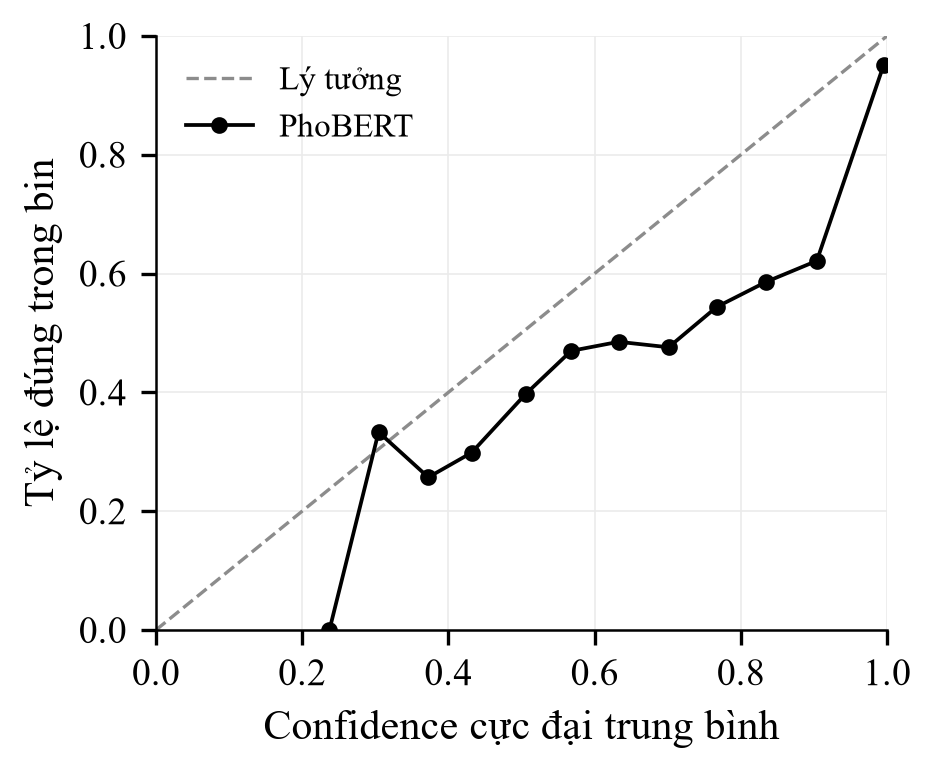
\includegraphics[width=\linewidth]{assets/compact/pho_reliability_before.png}\caption{Softmax chưa hiệu chỉnh.}\end{subfigure}\hfill
\begin{subfigure}[t]{.48\textwidth}\centering
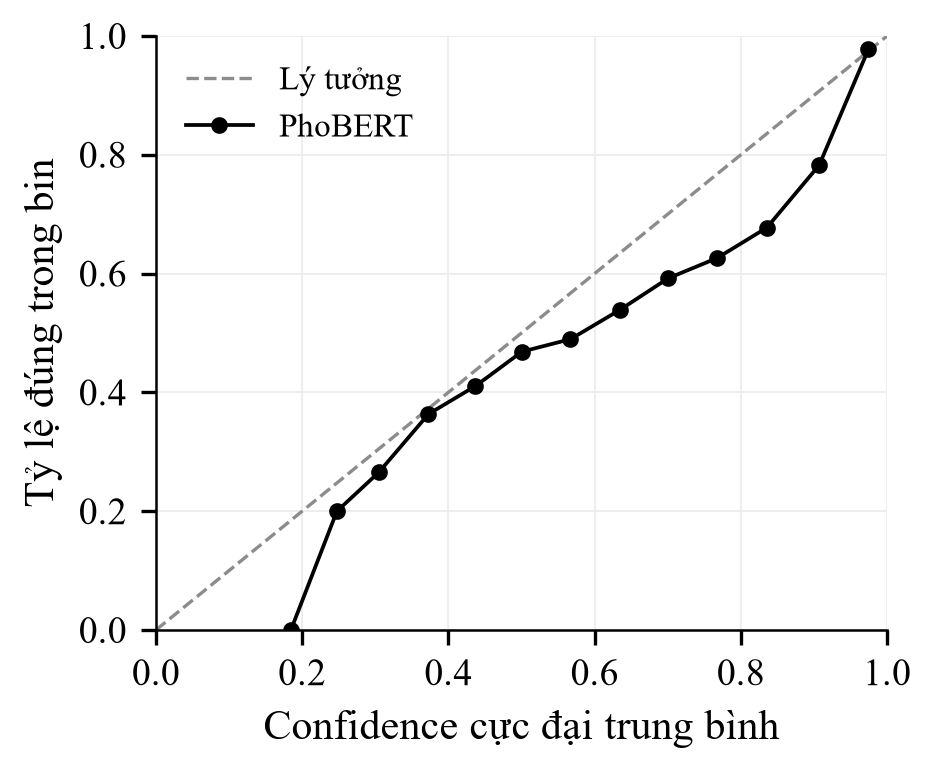
\includegraphics[width=\linewidth]{assets/compact/pho_reliability_after.png}\caption{Sau temperature scaling.}\end{subfigure}
\caption{Reliability PhoBERT trên cùng test, cùng thang trục và 15 bin; confidence cực đại trước hệ số quyết định theo lớp.}\label{fig:phobert-reliability}\end{figure}
ECE dùng 15 khoảng đều và correctness của argmax chuẩn; bin không rỗng đóng góp theo số mẫu. Quy ước mã nguồn có cận trên mở, nên xác suất đúng bằng 1 không nằm trong bin cuối; mẫu số là tổng bài thuộc các bin. ECE phụ thuộc cách chia khoảng và có thể che sai lệch ở lớp hiếm; không chứng nhận xác suất của từng bài.

Với PhoBERT, NLL giảm từ 0,383892 xuống 0,322030, ECE từ 0,060291 xuống 0,025071. Các giá trị mô tả $p(T)$, chưa xác nhận calibration của $q$ hoặc confidence nhãn cuối khi $\tau_c$ đổi nhãn. Việc áp dụng ngưỡng confidence cho tự động duyệt phải được kiểm tra theo chính luồng quyết định đó.

Phân tích selective prediction trên test cho thấy ngưỡng 0,75 giữ 27.644 bài (coverage 92,16\%), Accuracy nhóm 94,55\%; ngưỡng 0,95 giữ 22.322 bài (74,42\%) với Accuracy nhóm 98,36\%. Đây là Accuracy có điều kiện trên nhóm được giữ, không thay Accuracy toàn bộ test và không là hiệu quả sản xuất thực tế. Ngưỡng 0,99 không có mẫu đạt, nên Accuracy không xác định. Đường coverage--accuracy và chính sách routing được trình bày ở Phụ lục~\ref{app:application}.


\subsection{Vì sao NLL, ECE và F1 có thể khác thứ hạng}
NLL sử dụng xác suất của nhãn tham chiếu cho từng bài. Một dự đoán sai nhưng rất tự tin làm xác suất nhãn thật nhỏ và bị phạt mạnh; một quyết định đúng vẫn có thể có NLL cao nếu xác suất phân bố chưa tập trung vào nhãn đó. F1 không giữ mức độ tự tin, nên thay $T$ có thể cải thiện NLL mà F1 giữ nguyên. Đây là lý do không gọi temperature scaling là một lần train classifier để nâng Accuracy.

ECE tập hợp bài theo confidence cực đại rồi so trung bình confidence với tỷ lệ đúng trong bin. Sai lệch có thể được bù trong tổng hợp và số bin ảnh hưởng kết quả. Một model phân loại ít chính xác hơn vẫn có thể tự tin phù hợp với mức đúng thấp hơn, đạt ECE nhỏ. Vì thế, ECE BiLSTM/LR thấp hơn PhoBERT không phủ định thứ hạng Macro-F1; chúng đo những yêu cầu khác nhau của đầu ra.

Quy tắc $\tau_c$ có thể chọn nhãn không phải argmax xác suất, nên confidence dùng trong app cũng không luôn là cực đại. Chứng cứ reliability trước/sau temperature chỉ đánh giá phân bố $p(T)$ theo giao thức đã công bố. Nếu muốn dùng confidence của nhãn cuối cho auto-approve, cần kiểm tra lỗi và calibration trực tiếp ở luồng đó, theo lớp và thời điểm. Hiện các số mô phỏng coverage là mô tả test, không một ngưỡng bảo đảm cho dữ liệu vận hành.

\FloatBarrier
\section{Chi phí tính toán và trả lời RQ1--RQ3}

\DataTable{tables/comparison_timing.tex}{Thời gian được ghi trong artifact của từng pipeline; dấu -- ở PhoBERT nghĩa không có lượt tìm nhiều cấu hình tương ứng. Phạm vi timer cần đọc cùng diễn giải.}
SVM fit classifier được chọn trong 27,319 giây, LR trong 239,531 giây, đều dùng CPU với bốn luồng. Tổng tìm 12 cấu hình là 758,245 và 2.370,248 giây, gồm tạo TF--IDF và các lượt tối ưu. BiLSTM train cấu hình chọn trong 1.779,429 giây (29,66 phút), tìm ba cấu hình trong 4.473,369 giây (74,56 phút). PhoBERT fine-tuning bảy epoch mất 12.429,912 giây (207,17 phút), không tính chi phí tiền huấn luyện mô hình nền. Timer fit SVM/LR chỉ đo tối ưu classifier; timer huấn luyện neural gồm vòng train, validation theo epoch và lưu checkpoint, nên không phải các hạng chi phí hoàn toàn đồng nhất.

Phạm vi suy luận khác nhau. SVM/LR gồm TF--IDF transform và decision function trên CPU, không gồm phân đoạn tiếng Việt. BiLSTM gồm DataLoader, chuyển tensor sang GPU và forward, không gồm phân đoạn/mã hóa; batch test là 128. Timer test PhoBERT là 106,322 giây trên GPU, không gồm nạp model; batch test là 64 và input đã mã hóa. Các thời gian 12,689/13,125/9,233 giây của ba đối chứng phản ánh workload được ghi, không phải latency từ URL đến nhãn trong app. Chưa có benchmark serving CPU đồng nhất để xếp hạng độ trễ triển khai.

BiLSTM có 10,34 triệu tham số, PhoBERT 135,01 triệu; hai mô hình tuyến tính lưu hệ số, từ vựng và IDF, không có encoder lớn. Artifact BiLSTM ghi peak allocated 0,564 GiB trong huấn luyện cấu hình được chọn, metadata PhoBERT ghi 5,388 GiB ở lượt đánh giá. Hai mốc đo khác giai đoạn; chưa có peak RAM/VRAM toàn quy trình đồng nhất cho cả bốn model. Không dùng dung lượng file nén hoặc bộ nhớ CUDA reserved thay cho bộ nhớ thực thi được đo.



\subsection{Chi phí của biểu diễn và cập nhật tham số}
TF--IDF có chi phí đọc, đếm và biến đổi văn bản trước tối ưu classifier. Ma trận thưa giúp tính trên các phần tử có giá trị thay vì một tensor dense toàn bộ 150.000 chiều mỗi bài. Thời gian fit classifier chọn không chứa toàn bộ công việc tạo ra nó, nên một mốc CPU ngắn không đồng nghĩa pipeline từ corpus thô đến artifact chỉ mất từng đó giây. Tổng search có phạm vi rộng hơn và được trình bày riêng.

BiLSTM cập nhật embedding học từ train cùng recurrent/head; packed sequence tránh quét PAD nhưng vẫn có phụ thuộc trạng thái theo chiều thời gian. PhoBERT tạo các phép attention và FFN trên chuỗi 256, cập nhật backbone lớn đã tiền huấn luyện. Những khác biệt cơ chế giúp hiểu yêu cầu tính toán, nhưng chưa đủ phân rã chính xác số giây cho từng phép toán. Không dùng riêng chiều dài 512 từ và 256 subword để suy neural nào tất yếu nhanh hơn: hai đơn vị và phép tính khác nhau.

GPU batch processing trong evaluation dùng nhiều bài mỗi forward, trong khi app nhận request qua API và có thể chạy CPU. Một throughput lớn nhờ batch chưa bảo đảm độ trễ thấp khi bài đến lẻ hoặc hàng đợi dài. Các đo kiểm đồng nhất cần khóa lượng văn bản, preprocessor, batch, precision, thiết bị và điểm bắt đầu/kết thúc timer. Snapshot hiện tại cung cấp các timer của lượt thực nghiệm, chưa cung cấp toàn bộ phép đo serving này.


\subsection{Phạm vi đo và ý nghĩa đối với lựa chọn model}
Chi phí selected fit phù hợp câu hỏi dùng lại một cấu hình đã biết; tổng search phù hợp câu hỏi tài nguyên để chọn ra cấu hình đó. SVM/LR có số ứng viên bằng nhau nhưng solver và tiêu chí tối ưu khác, còn neural bao gồm validation và checkpoint theo epoch. Một ratio từ các timer này chỉ mô tả lượt chạy đã ghi, không là tốc độ tuyệt đối của một họ thuật toán. Tiền huấn luyện PhoBERT còn là chi phí bên ngoài lượt fine-tuning, chưa được tính vào bảng.

Phép đo evaluation inference theo batch cũng khác một yêu cầu phục vụ đơn. Trong app còn có trích xuất URL, tiền xử lý, mã hóa, transport, truy cập database và thời gian hàng đợi. Những bước không nằm trong timer offline không được suy bằng cách chia tổng giây cho số test rồi gọi latency HTTP. Container phục vụ CPU trong khi neural offline đo GPU, càng cần một benchmark cùng điều kiện trước khi kết luận model nào phục vụ nhanh nhất.

Tài nguyên lưu trữ và tài nguyên thực thi cũng khác nhau. File trọng số, từ vựng và tensor cache hỗ trợ tái hiện nhưng không đều phải nằm trên GPU khi forward. Số tham số cung cấp quy mô kiến trúc, chưa đo peak RAM toàn quy trình. Các mốc VRAM hiện có thuộc hai giai đoạn khác nhau; bảng không có số peak đồng nhất cho cả bốn pipeline và không tự bổ sung bằng ước lượng.

Một quyết định triển khai còn phụ thuộc hậu quả của lỗi từng lớp và khả năng rà soát. Chênh lệch Macro-F1 có thể đáng giá khi cải thiện chuyên mục khó quan trọng, nhưng không đủ nếu lỗi tự động ở một lớp hiếm gây chi phí lớn. Vì vậy, câu trả lời RQ2 giữ điều kiện đo và liên kết với RQ3, thay vì chuyển một thứ hạng F1 thành quyết định duy nhất cho mọi tải và chính sách.

\FloatBarrier

\subsection{Diễn giải theo câu hỏi nghiên cứu}

\textbf{RQ1:} trên snapshot và phép chia hiện tại, PhoBERT argmax có Macro-F1 cao nhất; SVM là đối chứng tuyến tính mạnh với chi phí fit thấp. Bất định ghép cặp ủng hộ khoảng cách PhoBERT với ba đối chứng khi giữ model cố định, nhưng không xác nhận thứ hạng SVM--LR--BiLSTM ở mọi lần train.

\textbf{RQ2:} mức tăng khoảng 1,89 điểm Macro-F1 so với SVM đi kèm fine-tuning GPU tốn thời gian hơn và encoder lớn hơn. Các timer cho phép nhận diện đánh đổi trong thực nghiệm, chưa tạo một phép đo latency/bộ nhớ serving hoàn toàn đồng nhất. Lựa chọn triển khai còn phụ thuộc tài nguyên, lưu lượng và yêu cầu rà soát, không chỉ một F1 tổng thể.

\textbf{RQ3:} khác biệt theo lớp có thật trong mẫu: BiLSTM/LR tốt hơn ở Nông thôn mới, PhoBERT tốt hơn rõ hơn ở Dân tộc thiểu số và miền núi, còn các lớp chủ đề tập trung dễ đạt điểm cao với TF--IDF. Lỗi chung ở ranh giới nhãn biên tập cho thấy cần đầu tư kiểm toán taxonomy và mẫu khó, không chỉ tăng độ phức tạp model.

Tất cả kết luận trên thuộc một nguồn báo, một seed và các pipeline đã công bố. Không có test tương lai/ngoài nguồn, thực nghiệm nhiều seed hoặc ablation cô lập pretraining, lặp tiêu đề, stopword và chiều dài. Kết quả không xác lập PhoBERT luôn tốt nhất trên tin tức tiếng Việt; ứng dụng minh họa tiếp tục dùng gói PhoBERT và chính sách hiệu chỉnh đã được kiểm chứng.
